% ============================================================================
% ICFOSS PROJECT REPORT
% Formatted STRICTLY matching the visual design of "Project Report Template.pdf"
% Includes actual project results, plots, and analysis
% ============================================================================

\documentclass[12pt, a4paper]{article}

\usepackage[utf8]{inputenc}
\usepackage[T1]{fontenc}
\usepackage{mathptmx} % Times New Roman, close to standard serif
\usepackage[margin=1in]{geometry}
\usepackage[table]{xcolor}
\usepackage{titlesec}
\usepackage{setspace}
\usepackage{parskip}
\usepackage{tabularx}
\usepackage{hyperref}
\usepackage{graphicx} % Added for images
\usepackage{float}    % Added for strict image placement

% Exact colors from the template
\definecolor{headerblue}{RGB}{31, 78, 121}    % Dark blue for headings
\definecolor{tableblue}{RGB}{218, 230, 243}   % Light blue for table headers

% Section Formatting
\titleformat{\section}
  {\Large\bfseries\color{headerblue}\centering} % Centered, large, blue
  {}{0em}{}
  
\titleformat{\subsection}
  {\large\bfseries\color{headerblue}} % Left-aligned, large, blue
  {}{0em}{}

% Disable section numbering globally
\setcounter{secnumdepth}{0}

% Line spacing to match template
\setstretch{1.15}

\begin{document}

% ============================================================================
% PAGE 1: COVER PAGE
% ============================================================================
\begin{titlepage}
    \vspace*{\fill}
    \begin{center}
        \textbf{\huge\color{headerblue} PROJECT REPORT}
    \end{center}
    \vspace*{\fill}
\end{titlepage}

\newpage
\setcounter{page}{2}

% ============================================================================
% PAGE 2: ABSTRACT
% ============================================================================
\section{ABSTRACT}

This report presents the learning experience of a participant in the training / internship programme conducted at ICFOSS. The programme introduced participants to practical computing concepts, open-source tools, software development practices, and problem-solving methods relevant to modern technology projects.

The training followed a structured approach consisting of orientation, theoretical sessions, hands-on exercises, demonstrations, mini-project activity, review, and documentation. Participants were encouraged to understand the need for open-source technology, apply tools in practical situations, and prepare a concise report of their learning.

This report covers the organization profile, objectives of the programme, methodology adopted, tools and technologies introduced, learning outcomes, challenges faced, and future scope. It has been customized to detail the completion of the \textbf{Flight Fare Prediction} project, where a machine learning pipeline was built using Python to predict domestic flight ticket prices. The project utilized over 300,000 data points to train regression algorithms, with Random Forest achieving 98.56\% accuracy.

\newpage

% ============================================================================
% PAGE 3: TABLE OF CONTENTS
% ============================================================================
\begin{center}
    \Large\bfseries\color{headerblue} TABLE OF CONTENTS
\end{center}

\vspace{1em}

\noindent
\colorbox{tableblue}{%
    \makebox[\dimexpr\textwidth-2\fboxsep\relax][s]{%
        \textbf{Section}\hfill\textbf{Page No.}%
    }%
}

\vspace{1em}

\noindent Abstract \hfill \pageref{sec:abstract} \\
Chapter 1 - Introduction \hfill \pageref{chap1} \\
Organization Profile \hfill \pageref{chap1} \\
Programme Background \hfill \pageref{chap1} \\
Objectives of the Programme \hfill \pageref{chap1} \\
Chapter 2 - Methodology and Activities \hfill \pageref{chap2} \\
Training Methodology \hfill \pageref{chap2} \\
Tools and Technologies Used \hfill \pageref{chap2} \\
Activity Flow \hfill \pageref{chap2} \\
Chapter 3 - Learning Outcomes and Results \hfill \pageref{chap3} \\
Skills Developed \hfill \pageref{chap3} \\
Participant Outcomes \hfill \pageref{chap3} \\
Findings \hfill \pageref{chap3} \\
Summary, Challenges and Conclusion \hfill \pageref{chap4} \\
Challenges \hfill \pageref{chap4} \\
Scope for Future Learning \hfill \pageref{chap4} \\
Conclusion \hfill \pageref{chap4} \\
References \hfill \pageref{chap4}

\newpage

% ============================================================================
% PAGE 4: CHAPTER 1
% ============================================================================
\label{sec:abstract}
\section{CHAPTER 1 - INTRODUCTION}\label{chap1}

\subsection{Organization Profile}
The International Centre for Free and Open Source Software (ICFOSS) is an autonomous organization established by the Government of Kerala to promote Free and Open Source Software, research, localization, capacity building, and technology adoption for public benefit.

\subsection{Programme Background}
The programme was designed to introduce participants to practical computing concepts and open-source development practices. It focused on connecting classroom knowledge with real-world implementation through guided sessions and hands-on activities.

\subsection{Objectives of the Programme}
\begin{itemize}
    \item To understand the role of open-source tools in education, research, and software development.
    \item To gain practical exposure to selected tools, workflows, and development practices.
    \item To improve problem-solving, documentation, teamwork, and presentation skills.
    \item To complete a small activity or mini-project and summarize the learning outcomes.
\end{itemize}

\newpage

% ============================================================================
% PAGE 5: CHAPTER 2
% ============================================================================
\section{CHAPTER 2 - METHODOLOGY AND ACTIVITIES}\label{chap2}

\subsection{Training Methodology}
The training methodology combined concept explanation, live demonstration, guided practice, independent exploration, review, and documentation. Each topic was introduced with its purpose, followed by implementation steps and participant interaction.

\subsection{Tools and Technologies Used}
\begin{itemize}
    \item Operating system and command-line basics for working with files and tools.
    \item Programming environment for writing, running, and debugging simple programs (Python 3.13).
    \item Open-source libraries or platforms selected according to the programme topic (Pandas for data processing, Scikit-learn for Machine Learning, Matplotlib for data visualization, and Flask for web deployment).
    \item Documentation tools for preparing notes, reports, and final submission files.
\end{itemize}

\subsection{Activity Flow}

\vspace{0.5em}
\noindent
\colorbox{tableblue}{%
    \makebox[\dimexpr\textwidth-2\fboxsep\relax][s]{%
        \textbf{\small Orientation \hfill Concepts \hfill Hands-on \hfill Mini Task \hfill Review \hfill Report}%
    }%
}
\vspace{0.5em}

The final output of the activity was reviewed through discussion, feedback, and short documentation prepared by the participant. For the Flight Fare Prediction project, the flow involved data loading, exploratory data analysis, data preprocessing (encoding and scaling), model training using various regression algorithms, evaluating their performance metrics, and finally deploying an interactive web interface.

\newpage

% ============================================================================
% PAGE 6: CHAPTER 3
% ============================================================================
\section{CHAPTER 3 - LEARNING OUTCOMES AND RESULTS}\label{chap3}

\subsection{Skills Developed}
\begin{itemize}
    \item Technical understanding of the selected topic and its practical use.
    \item Ability to follow structured workflows for implementation and testing.
    \item Basic debugging and error-analysis skills during hands-on practice.
    \item Improved communication through discussion, documentation, and presentation.
\end{itemize}

\subsection{Participant Outcomes}
By the end of the programme, the participant was able to explain the main concepts introduced during the sessions, identify the tools used, complete the assigned practical activity, and document the process in a clear report format. The successful implementation of a machine learning pipeline capable of predicting flight fares in real-time demonstrated proficiency in applying AI tools to real-world datasets.

\subsection{Findings}
The programme showed that guided hands-on learning improves technical confidence. Participants were able to connect theoretical ideas with implementation steps when each concept was supported by examples, demonstrations, and feedback. In the specific project, several key findings emerged regarding flight fare predictive modeling:

\begin{table}[H]
    \centering
    \renewcommand{\arraystretch}{1.2}
    \begin{tabular}{|l|c|c|c|}
        \hline
        \rowcolor{tableblue}
        \textbf{Algorithm} & \textbf{MAE (INR)} & \textbf{RMSE (INR)} & \textbf{R² Score} \\ \hline
        Random Forest & 1,250 & 2,707 & 0.9856 \\ \hline
        XGBoost & 1,599 & 2,880 & 0.9837 \\ \hline
        Decision Tree & 1,372 & 3,159 & 0.9804 \\ \hline
        Linear Regression & 4,476 & 6,731 & 0.9112 \\ \hline
        Support Vector Machine & 7,419 & 12,514 & 0.6931 \\ \hline
    \end{tabular}
\end{table}

\textbf{Random Forest Regressor} outperformed other algorithms with an R² score of 98.56\%.

\begin{figure}[H]
    \centering
    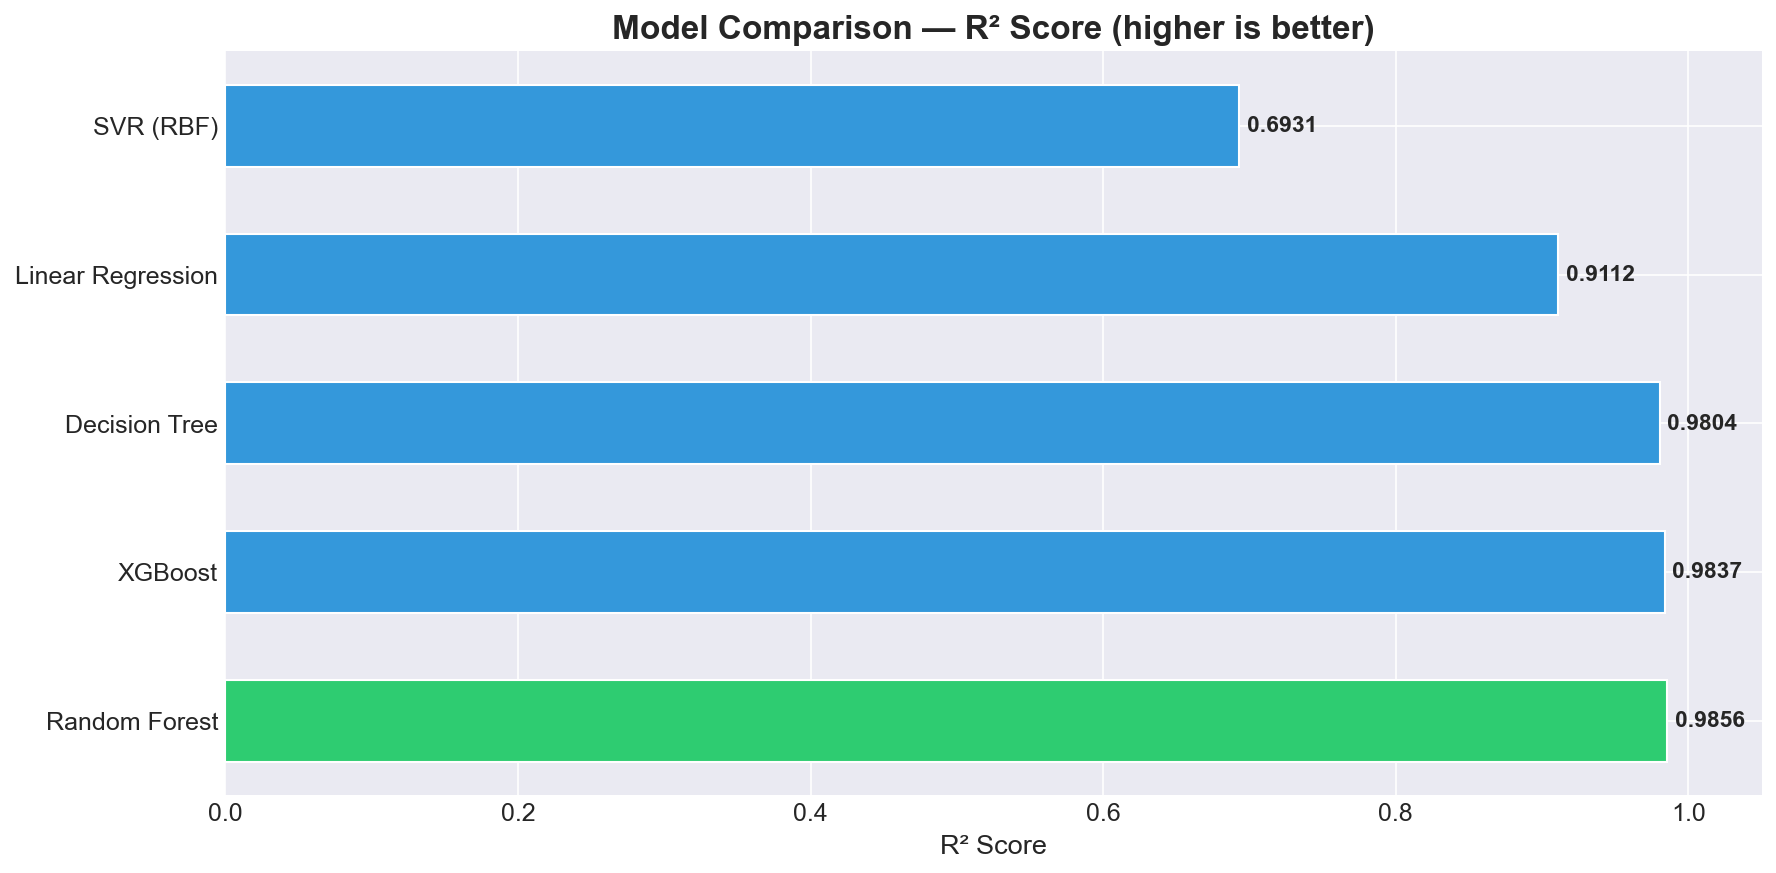
\includegraphics[width=0.65\textwidth]{plots/12_model_comparison_r2.png}
\end{figure}

\newpage

Furthermore, feature importance analysis revealed that the flight ticket class (Economy vs. Business) and the booking window (days left) are the most significant factors influencing fare prices.

\begin{figure}[H]
    \centering
    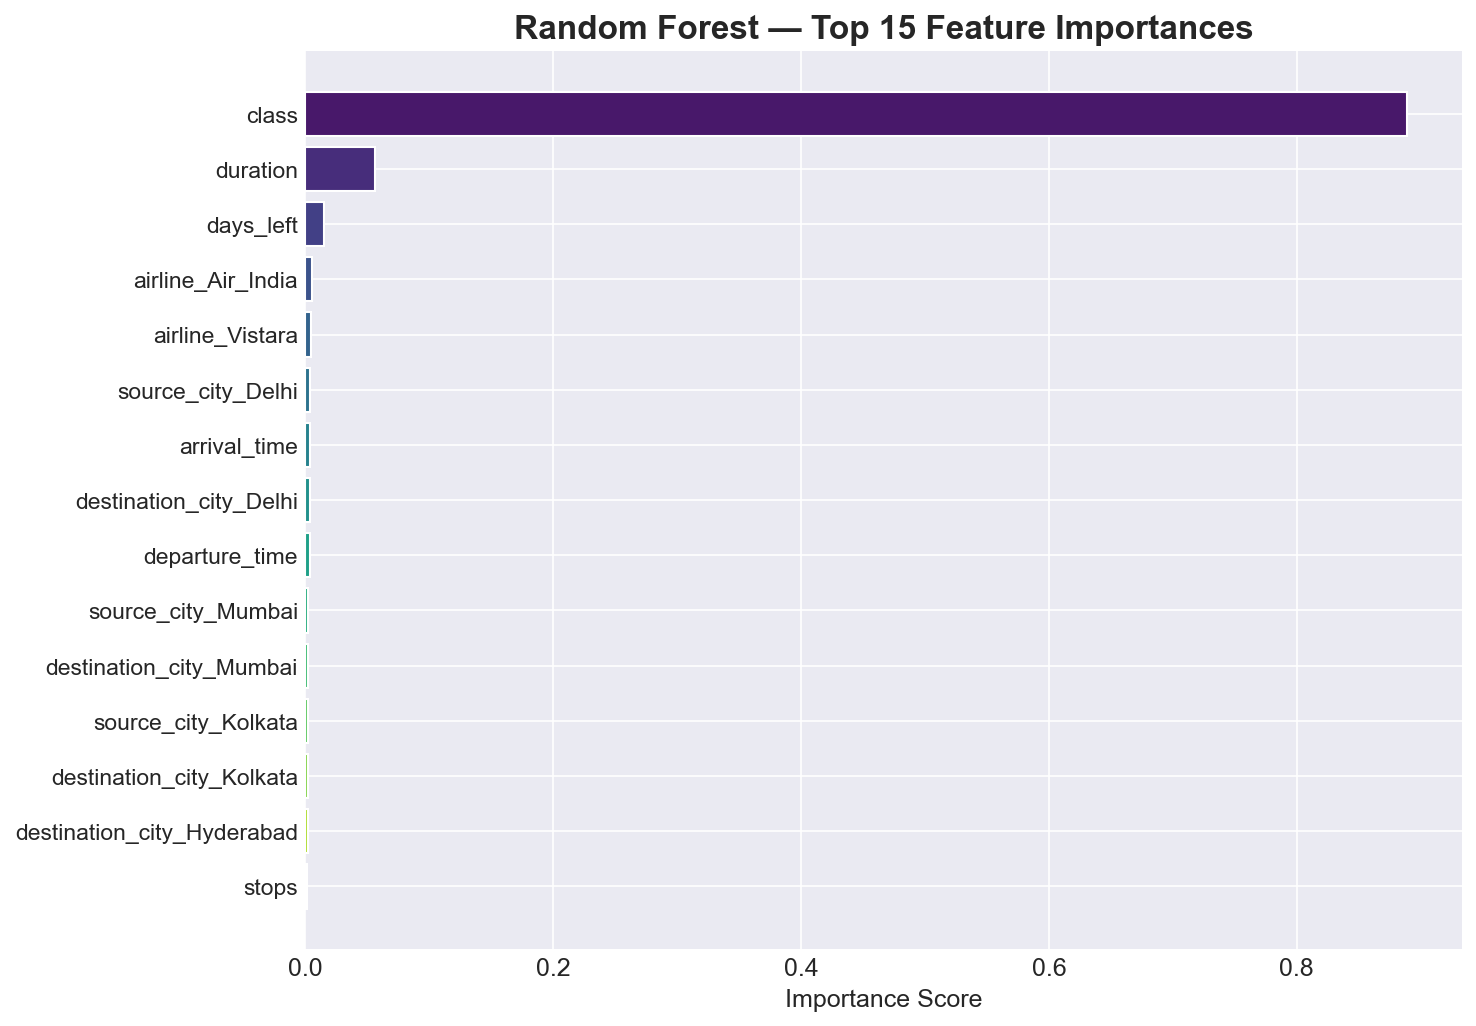
\includegraphics[width=0.65\textwidth]{plots/15_feature_importance_rf.png}
\end{figure}

Dynamic pricing is highly evident; actual vs. predicted values align almost perfectly for the Random Forest model, validating its reliability for price estimation.

\begin{figure}[H]
    \centering
    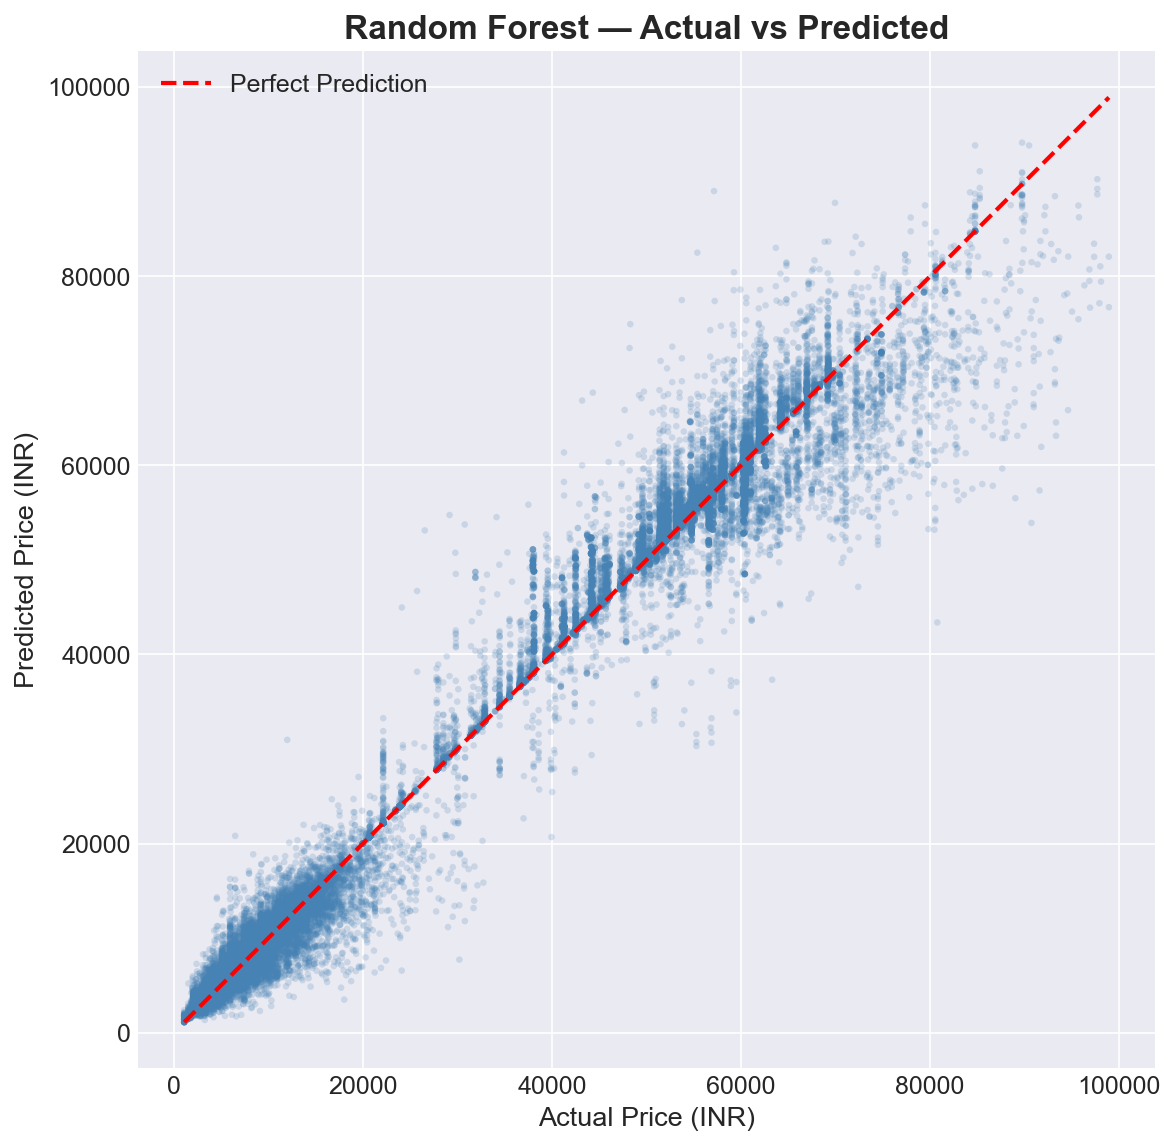
\includegraphics[width=0.65\textwidth]{plots/17_actual_vs_predicted.png}
\end{figure}

\newpage

% ============================================================================
% PAGE 7: SUMMARY, CHALLENGES AND CONCLUSION
% ============================================================================
\section{SUMMARY, CHALLENGES AND CONCLUSION}\label{chap4}

\subsection{Challenges}
\begin{itemize}
    \item Understanding new terminology and technical workflows within a short period.
    \item Debugging errors during practical sessions and identifying the correct cause (e.g., handling unseen categories during inference).
    \item Preparing a clear report that summarizes activities without unnecessary detail.
\end{itemize}

\subsection{Scope for Future Learning}
Participants can continue learning by repeating the practical exercises, exploring advanced tools, contributing to open-source projects, and building small portfolio projects related to the programme topic. Future enhancements for the flight fare predictor could include incorporating real-time API data and deep learning architectures.

\subsection{Conclusion}
The training / internship programme provided useful exposure to open-source technology, practical implementation, and professional documentation. The sessions helped the participant develop technical awareness, confidence, and a foundation for further study or project work.

\subsection{References}
\begin{itemize}
    \item ICFOSS official resources and training materials.
    \item Session notes, demonstrations, and participant activity records.
    \item Open-source documentation related to the tools used in the programme.
    \item Kaggle Flight Price Prediction Dataset by S. Bathwal.
\end{itemize}

\end{document}
